\chapter{Slowly decaying eigenmodes\label{chap:currents}}
\thispagestyle{chapterBeginStyle}

In the previous chapter, we have numerically shown the existence of optimal anisotropy
\(\Delta_{O} = \exp(- \alpha + 2)\), which ensures slow relaxation of the spin current
 \(j^{\sigma}\)~\eqref{eq:spin_current} and consequently quasiballistic spin transport.
 Here, we will demonstrate that this feature is not unique to the spin current, but
 exhibited also by a class of other, \textit{local} operators. To this end, we will
 employ an algorithm devised by \textcite{Mierzejewski2015a}, originally designed to
 identify local integrals of motion in integrable tight-binding models. As the model
 we are considering in this work is not integrable, we are not expecting to find
 strictly conserved quantities, but only so-called \textbf{local slowly relaxing
 operators (LSROs)}. We will interpret the discovered observables in terms of
 fermionic currents, describing particle hopping with various ranges.
 Moreover, we will also show how to improve the numerical efficiency of
 the algorithm, by utilizing symmetry subspaces and the Dynamical Quantum Typicality
 approach to correlation functions\footnote{And why it, unfortunately, fails in this case.}
(cf. section~\ref{sec:DQT}).


\section{Detecting local slowly relaxing operators \label{sec:slowly_relaxing_operators}}
\subsection{Theoretical description}
Let us start by introducing in detail the original algorithm for detecting local integrals
of motion (LIOMs), following the original article by~\autocite{Mierzejewski2015a}.
In principle, finding a \textbf{complete set of LIOMs} is a conceptually
nontrivial task, however, this procedure reduces it to a simple application of linear algebra~\autocite{Mierzejewski2015a}.
In this section, unless stated otherwise, by \(H\) we will denote an arbitrary
tight-binding Hamiltonian with periodic boundary conditions
on \(L\) sites, having eigenstates \(H \ket{n} = \epsilon_{n} \ket{n}\). Moreover,
for any operator \(A\) we define \(A_{mn} \equiv \matrixel{m}{A}{n}\).

In order to employ techniques from linear algebra, we need to have a linear space of some kind.
This role is played by the space of \textit{local, traceless, and translationally invariant} operators,
supported on up to \(M\) sites and acting on vectors from a Hilbert space \(\mathcal{H}\) of 
dimension \(\mathcal{D}\). We will denote this space by \(\mathcal{V}_{M}\). Its building blocks are the
spaces \(\mathcal{V}^m\), of operators supported on exactly \(m\) sites, i.e. of the form
\begin{center}
    \hspace*{-0.5cm}
    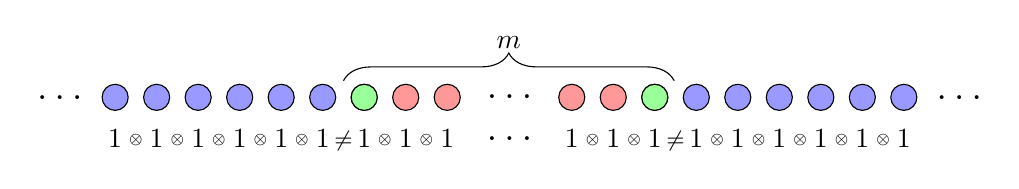
\begin{tikzpicture}[node distance = 15pt, auto]
        \tikzstyle{line} = [draw, -latex',thick]
        \tikzstyle{site1}=[circle, draw, fill=blue!40]
        \tikzstyle{site2}=[circle, draw, fill=red!40]
        \tikzstyle{site3}=[circle, draw, fill=green!40]
        % Place nodes
    
        \node [site1] (site-1) at (-8, 0) {};
        \foreach \x / \name in {1/2,2/3,3/4,4/5,5/6}
        \node [site1, right of=site-\x] (site-\name) {};
    
        \node [site2, right of =site-6] (site-7){};
        \foreach \x / \name in {7/8,8/9}
        \node [site2, right of=site-\x] (site-\name) {};
    
        \node [site2, right of=site-9, node distance=45pt] (site-10){};
        \foreach \x / \name in {10/11,11/12}
        \node [site2, right of=site-\x] (site-\name) {};
    
        \node[site1, right of=site-12] (site-13){};
        \foreach \x / \name in {13/14,14/15,15/16,16/17,17/18}
        \node [site1, right of=site-\x] (site-\name) {};
    
        \node [left of=site-1, node distance=20pt] {\Large $ \ldots $};
        \node [right of=site-18, node distance=20pt] {\Large $ \ldots $};
    
        \node [site3, right of=site-6] (site-X) {};
        \node [site3, right of=site-11] (site-X) {};
    
        \foreach \x in {1,...,18}
        \node [black, below of=site-\x](op-\x) {\(\mathbb{1}\)};
    
        \foreach \x / \y in {1/2,2/3,3/4,4/5,5/6,7/8,8/9,10/11,11/12,13/14,14/15,15/16,16/17,17/18}
        \path[draw=none] (op-\x) -- (op-\y) node [black,midway,yshift=-6pt] {\tiny$\otimes$};
    
        \path[draw=none] (op-6) -- (op-7) node [black,midway,yshift=-8pt] {\footnotesize$\neq$};
        \path[draw=none] (op-12) -- (op-13) node [black,midway,yshift=-8pt] {\footnotesize$\neq$};
        % \foreach \x in {-1.5,-1.0,-0.5,0.5,1.0,1.5}
        % \node [site2] (site-\x) at (\x, 0) {};
    
        \draw [decorate,decoration={brace,amplitude=10pt},yshift=6pt]
        (-5.1,0) -- (-0.9,0) node [black,midway,yshift=8pt] {$m$};
    
        \path [draw=none] (site-9) -- (site-10) node [black,midway,yshift=-4pt] {\Large$\ldots$};
        \path [draw=none] (op-9) -- (op-10) node [black,midway,yshift=-4pt] {\Large$\ldots$};
      \end{tikzpicture}    
\end{center}    
where blue circles correspond to single-site identity operators, green circles to an arbitrary
single-site operator except for the identity and red circles to an arbitrary single-site operator.
If we were to allow identity operators on green sites, we would have obtained a \((m-1)\)-local operator.
It is easy to see that an arbitrary linear combination of operators from \(\mathcal{V}^m\) is again
an element of \(\mathcal{V}^m\), hence \(\mathcal{V}^m\) is a linear space. Therefore,
the full space
\begin{equation}
    \mathcal{V}_{M} = \bigoplus_{m=1}^{M} \mathcal{V}^m
\end{equation}
is also a linear space. We will always assume that \(0\leq M \leq L/2\).

Using the infinite temperature correlation function (cf. Eq.~\eqref{eq:corr_fun}) we can endow this space with an inner product
\begin{equation}
    \mathcal{V}_M \cross \mathcal{V}_M \ni (A, B) \mapsto \hs{A}{B}
    \equiv \frac{1}{\mathcal{D}}\Tr\left(AB\right) = \frac{1}{D}\sum_{n,m = 1}^{D} A_{nm} B_{nm}^{\ast} \in \CC
    \label{eq:hs_prod}
\end{equation}
called the \textbf{Hilbert-Schmidt inner product} and
inducing the \textbf{Hilbert-Schmidt norm} \(\norm{A} = \sqrt{\hs{A}{A}}\). It is worth noting, that
if we let the first operator be time-dependent, and consider the Hilbert-Schmidt inner product
as a function of time, we obtain the infinite temperature correlation function~\eqref{eq:corr_fun}.
Because we only consider finite systems in this thesis, we do not need to worry about
situations where the trace is not well defined. The pair \( (\mathcal{V}_M, \hs{\cdot}{\cdot}) \)
is then a finite-dimensional Hilbert space.
We are now able to state more precisely what we mean by a complete set of LIOMs.
It is a set of local operators \(\{Q_{\beta} : \comm{Q_{\beta}}{H} = 0\}\), such that
for any observable \(A\) we have
\begin{equation}
    \lim_{t\to\infty} \hs{A(t)}{A} = \sum_{\beta} \frac{\hs{Q_{\beta}}{A}^2}{\hs{Q_{\beta}}{Q_{\beta}}}
\end{equation}
i.e. the completeness is understood as the saturation of the Mazur bound~\autocite{Mazur1969}.

The mathematical stage is now set, so let us proceed further toward the algorithm. 
As \(\mathcal{V}_M\) is a linear space, it possesses a basis \(\{O_{\alpha}\}\),
which with the help of the inner product can be made into an orthonormal basis \(\hs{O_{\alpha}}{O_{\alpha^{\prime}}} = \delta_{\alpha\alpha^{\prime}}\).
We can also think of this space as an orthogonal subspace of the space \(\mathcal{V}\) of all possible operators
acting on \(\mathcal{H}\), in the sense that
\begin{equation}
    \big(\forall A \in \mathcal{V} \big) \big( A = A^M + A^{\perp} = \sum_{\alpha} \hs{O_{\alpha}}{A} O_{\alpha} + A^{\perp}\big) ,
    \text{ such that } \big(\forall \alpha\big) \big( ({O_{\alpha}}|{A^{\perp}}) = 0\big)
    \label{eq:decomposition}
  \end{equation}
We will describe an example of such a basis in the next section, but for now, it is enough that it exists.

Next, we would like to determine the conserved part of all the basis operators \(O_{\alpha}\). We do this
by considering the infinite time average 
\begin{align}
    \bar{O}_{\alpha} = \lim_{\tau\to\infty}\frac{1}{\tau} \int_0^{\tau} \mathrm{d}t\, O_{\alpha}(t) &= 
     \lim_{\tau\to\infty}\frac{1}{\tau} \int_0^{\tau} \mathrm{d}t\, \mathrm{e}^{i H t}O_{\alpha} \mathrm{e}^{-i H t} \nonumber\\
     &= \sum_{m,n} (O_{\alpha})_{mn}\ketbra{m}{n} \lim_{\tau\to\infty} \frac{1}{\tau} \int_0^{\tau} \mathrm{d}t \, \mathrm{e}^{i(\epsilon_m-\epsilon_n)t} \nonumber\\
    &= \sum_{\substack{n,m \\ \epsilon_n = \epsilon_m}} (O_{\alpha})_{mn}\ketbra{m}{n}
    \label{eq:time_avg}
\end{align}
This time-averaging amounts to a cut-off, removing all matrix elements between non-degenerate eigenstates
of the Hamiltonian. A crucial property of this operation is that it is an orthogonal projection
in the space of operators, i.e. \(\hs{\bar{O}_{\alpha}}{\bar{O}_{\alpha^{\prime}}} = \hs{\bar{O}_{\alpha}}{O_{\alpha^{\prime}}}\). This will
in the end will allow us to distinguish between different types of conserved quantities.
However, our ultimate goal concerns LSROs in a system that is not integrable, which dictates the
need for performing also a finite-time averaging. Unfortunately, a simple omission of the limit
in Eq.~\eqref{eq:time_avg} destroys the projective character of this operation. To remedy this,
we introduce a parameter \(\tau\) and define effective time averaging~\autocite{Mierzejewski2015}
as
\begin{equation}
    \bar{O}_{\alpha}^{\tau} = \int_{-\infty}^{\infty} \mathrm{d}t\, O_{\alpha}(t) \frac{\sin(t/\tau)}{\pi t}
\end{equation}
By considering the Fourier transform of the \(\sin(x)/x\) function, it can be shown that
this expression is equivalent to (see Appendix~\ref{app:fourier} for details)
\begin{equation}
    \bar{O}_{\alpha}^{\tau} = \sum_{n,m} \underbrace{\theta\left(\frac{1}{\tau} - |\epsilon_n - \epsilon_m|\right)}_{\theta_{mn}^{\tau}} (O_{\alpha})_{mn} \ketbra{m}{n}
\label{eq:finite_time_avg}
\end{equation}
and because for Heaviside theta function we have \(\theta(x)^2 = \theta(x)\), the projective character is restored. 
Properties the \(\theta\)-function ensure that the \(\tau\to\infty\) limit of Eq.~\eqref{eq:finite_time_avg}
agrees with Eq.~\eqref{eq:time_avg}. Notice also the similarity of this expression to the integrated conductivity~\eqref{eq:integrated_conductivity}.
Indeed, the parameter \(1/\tau\) can be interpreted as \(\Omega\), giving the frequency cut-off for the matrix elements.
Thus, for finite \(\tau\), \(\hs{\bar{O}_{\alpha}^{\tau}}{\bar{O}_{\alpha^{\prime}}^{\tau}}\) can be related to the low-frequency spectrum of 
the correlation function \(\langle O_{\alpha}(t) O_{\alpha^{\prime}} \rangle\). We shall return to this idea later on.

Let us now calculate the commutator of \(O_{\alpha}^{\tau}\) with the Hamiltonian
\begin{align}
    \comm{H}{\bar{O}_{\alpha}^{\tau}} & = \sum_n \sum_{k,p} \epsilon_n \theta_{kp}^{\tau} (\bar{O}_{\alpha})_{kp} \comm{ \ketbra{n}{n}}{ \ketbra{k}{p}} \nonumber         \\
                             & = \sum_{k,p} \left(\epsilon_k-\epsilon_p\right) \theta_{kp}^{\tau} (\bar{O}_{\alpha})_{kp} \ketbra{k}{p} \xrightarrow{\tau \to \infty} 0 
        \label{eq:time_averaged_commutator}
\end{align}
We see that the operator obtained from infinite-time averaging is an integral of motion. Unfortunately,
this procedure modifies the support of the operator and in general \(\bar{O}_{\alpha} \not\in \mathcal{V}_M\), i.e. its locality is lost.

Having calculated the time-averaged basis \( \{\bar{O}_{\alpha}^{\tau}\} \), we would like to perform in a 
systematic way the decomposition~\ref{eq:decomposition}. We need the overlaps between the basis operators
before and after the time-averaging. Because of the projective character of the time-averaging, they are
given by the pairwise inner products of the time-averaged operators, which we collect into a matrix
\(K^{\tau}\), with elements
\begin{equation}
    K^{\tau}_{\alpha\alpha^{\prime}} = \hs{\bar{O}_{\alpha}^{\tau}}{\bar{O}_{\alpha^{\prime}}^{\tau}} = \sum_{n,m} \theta_{mn}^{\tau} (O_{\alpha})_{nm} (O_{\alpha^{\prime}})_{nm}^{\ast}
    \label{eq:overlap_matrix}
\end{equation}
This matrix is Hermitian by design, and in the case of systems with time-reversal symmetry, it is also real,
thus symmetric. By the spectral theorem, there exists a unitary matrix \(U\) that transforms it
via a similarity transformation to a diagonal matrix \(D\)
\begin{align}
    &\sum_{\alpha,\alpha^{\prime}} U_{\beta \alpha} K_{\alpha\alpha^{\prime}}^{\tau} U_{\beta^{\prime} \alpha^{\prime}}^{\ast}=\delta_{\beta\beta^{\prime}} \lambda_{\beta} \in
     \RR,\;\;\; \lambda_{\beta} \text{ --- eigenvalue of }K^{\tau} \label{eq:property diag} \\
    &UU^{\dag} = U^{\dag}U = \mathbb{1} \implies \sum_{\alpha} U_{\beta\alpha}U_{\beta^{\prime}\alpha}^{\ast} =
     \delta_{\beta\beta^{\prime}} \label{eq:propery_ortho}\\
    & U K^{\tau} = D U \implies \sum_{\alpha} U_{\beta\alpha} K_{\alpha\alpha^{\prime}}^{\tau} = \sum_{\alpha}  \delta_{\beta\alpha} \lambda_{\alpha} U_{\alpha\alpha^{\prime}} = \lambda_{\beta} U_{\beta\alpha^{\prime}}\label{eq:property}
  \end{align} 
Using the columns of \(U\), which are just the eigenvectors of \(K^{\tau}\), we can construct a new set of operators
\begin{equation}
    Q_{\beta} = \sum_{\alpha} U_{\beta \alpha} \bar{O}_{\alpha}^{\tau}
    \label{eq:liom}
\end{equation}
Let us note a few properties of the newly defined quantities. First, they are orthogonal
\begin{align}
    \hs{Q_\beta}{Q_{\beta^{\prime}}} &= \sum_{\alpha,\alpha^{\prime}} U_{\beta\alpha} {\hs{\bar{O_{\alpha}}^{\tau}}{\bar{O_{\alpha^{\prime}}}^{\tau}}} U_{\beta^{\prime}\alpha^{\prime}}^{\ast} 
    = \sum_{\alpha^{\prime}} \left(\sum_{\alpha}U_{\beta\alpha} K_{\alpha\alpha^{\prime}}^{\tau}\right)  U_{\beta^{\prime}{\alpha^{\prime}}}^{\ast}\nonumber \\ 
    &= \lambda_{\beta} \sum_{\alpha^{\prime}} U_{\beta\alpha^{\prime}} U_{\beta^{\prime}\alpha^{\prime}}^{\ast} = \lambda_{\beta} \delta_{\beta\beta^{\prime}}
  \end{align}
where the last two equalities follow from~\eqref{eq:property} and~\eqref{eq:propery_ortho} respectively.
From the fact that \(\hs{Q_{\beta}}{Q_{\beta}} = \lambda_{\beta}\) and that \(\hs{\cdot}{\cdot}\) is an inner product,
we immediately deduce that \(K^{\tau}\) is positive semidefinite.
We are now ready to consider the desired decomposition into the part that is supported on at most \(M\) sites and the remaining, nonlocal part
\begin{align}
    Q_{\beta} &=  \sum_{\alpha} \hs{O_{\alpha}}{Q_{\beta}}O_{\alpha} + Q_{\beta}^{\perp} = \sum_{\alpha,\alpha^{\prime}} U_{\beta \alpha^{\prime}}\hs{O_{\alpha}}{\bar{O}_{\alpha^{\prime}}^{\tau}}
    O_{\alpha}+Q_{n}^{\perp} \nonumber \\
    &= \sum_{\alpha,\alpha^{\prime}} U_{\beta\alpha^{\prime}}\hs{\bar{O}_{\alpha}^{\tau}}{\bar{O}_{\alpha^{\prime}}^{\tau}} O_{\alpha}+Q_{\beta}^{\perp}
    = \sum_{\alpha,\alpha^{\prime}} U_{\beta\alpha^{\prime}}K_{\alpha\alpha^{\prime}} O_{\alpha}+Q_{\beta}^{\perp} \nonumber \\
    &= \sum_{\alpha}  \left( \sum_{\alpha^{\prime}} U_{\beta\alpha^{\prime}}K_{\alpha\alpha^{\prime}}^{\tau}\right) O_{\alpha}+Q_{\beta}^{\perp} = \sum_{\alpha} 
    \lambda_{\beta} U_{\beta \alpha} O_{\alpha}+Q_{\beta}^{\perp} = Q_{\beta}^{M}+Q_{\beta}^{\perp}
    \label{eq:decomposition2}
  \end{align}
  Everything we did so far holds for an
arbitrary value of \(\tau\). However, let us for a moment restrict it to \(\tau\to \infty\).
This guarantees that the operators \(Q_{\beta}\) are integrals of motion.
  We have one step left to complete the algorithm and obtain a classification scheme for the
  integrals of motion. We need to determine how much of the operator \(Q_n\) is contained in the
  \(M\)-local part \(Q_{\beta}^M\). In other words, we want to calculate \(\norm*{Q_{\beta}^{\perp}}\).
  Consider the following calculation
  \begin{align}
    \lambda_{\beta} &= \hs{Q_{\beta}}{Q_{\beta}} = \hs{Q_{\beta}^M + Q_{\beta}^{\perp}}{Q_{\beta}^M + Q_{\beta}^{\perp}} = \hs{Q_{\beta}^M}{Q_{\beta}^M} +
     \hs{Q_{\beta}^{\perp}}{Q_{\beta}^{\perp}} + \underbrace{2 \hs{Q_{\beta}^M}{Q_{\beta}^{\perp}}}_{=0} \nonumber \\
     &= \hs{\sum_{\alpha} \lambda_{\beta} U_{\beta\alpha} O_{\alpha}}{\sum_{\alpha^{\prime}} \lambda_{\beta} U_{\beta\alpha^{\prime}} O_{\alpha^{\prime}}} + \norm{Q_{\beta}^{\perp}}^2 =
    \lambda_{\beta}^2 \sum_{\alpha,\alpha^{\prime}} U_{\beta\alpha} \hs{O_{\alpha}}{O_{\alpha^{\prime}}} U_{\beta\alpha^{\prime}}^{\ast} + \norm{Q_{\beta}^{\perp}}^2  \nonumber \\
    &=\lambda_{\beta}^2 + \norm{Q_{\beta}^{\perp}}^2
  \end{align}
  Rearranging the terms, we obtain the desired formula
  \begin{equation}
    \norm{Q_{\beta}^{\perp}}^2 = \lambda_{\beta}^2 - \lambda_{\beta} = \lambda_{\beta} (\lambda_{\beta} - 1) \geq 0
    \label{eq:liom_norm}
  \end{equation}
Thus, the spectrum of the matrix \(K\) is contained in the interval \([0,1]\) and
 determines the classification of the integrals of motion. We have three classes:
 \begin{itemize}
    \item local: \(\lambda_{\beta} = 1 \implies \norm{Q_{\beta}^{\perp}} = 0 \implies Q_{\beta} \in \mathcal{V}_M\)
    \item quasilocal: \(\lambda_{\beta} \in \left(0,1\right) \implies \norm{Q_{\beta}^{\perp}} > 0 \implies Q_{\beta} \in \mathcal{V} \)
    \item generic nonlocal: \(\lambda_{\beta} = 0 \implies \norm{Q_{\beta}} = 0\)
  \end{itemize}
  Let us now give a physical interpretation of these results. The procedure outlined above
  can be carried out for, in principle, arbitrary but finite systems size \(L\). However,
  to understand the character of the integrals of motion, we need to take the thermodynamic
  limit \(L\to\infty\). In practical calculations, we are always limited to finite, \(M\)-local basis
  of operators. Thus, the output of the algorithm is not the set of true integrals of motion \(\{Q_{\beta}\}\),
  but rather the set \(\{Q_{\beta}^M/\lambda_n\} \equiv \{I_{\beta}\}\) (as eigenvectors obtained from numerical
  procedures are usually normalized). If a particular \(\lambda_{\beta} = 1\), this
  is not a problem, as we have \(\norm*{Q^M_{\beta}} = 1\), and the true LIOM is \(M\)-local. However, if 
  for a given \({\beta}\) we have \(0 < \lambda_{\beta} < 1\), then \(\norm*{Q^M_{\beta}} < 1\). It is only if this norm
  stays non-zero in the thermodynamic limit, we can say that the operator is quasilocal. Then the \(Q_{\beta}^M\)
can be regarded as an \(M\)-local approximation of the true LIOM \(Q_{\beta}\).
  Numerous studies have confirmed their relevance in the theory of integrable 
  systems~\autocite{Ilievski2015, Ilievski2015b, Prosen2013, Prosen2014},
  however, we shall not deal with them any further. In fact, we shall not even deal with LIOMs, as
  the system we are interested in here is not integrable. Nevertheless, even without integrability,
  this algorithm will produce a sequence of operators \(\{I_{\beta}\}\), with the largest possible norm,
  often called \textbf{stiffness}. We will refer to them as \textbf{local slowly relaxing operators (LSROs)}
  and they will play a central role in section~\ref{sec:fermionic_currents}. We shall also relax the restriction
  \(\tau\to\infty\) and look at the LSROs at finite values of \(\tau\).

\subsection{Details of implementation}
Before proceeding further toward a concrete application of the procedure outlined above, let us first discuss
 some technical details of its implementation. The most demanding part, from the computational point of view,
 is the calculation of matrix elements~\eqref{eq:overlap_matrix}. It requires explicit construction of
 matrices of all the basis operators \(O_{\alpha}\), change of basis using Hamiltonian eigenstates,
 time averaging~\eqref{eq:finite_time_avg}, and finally carrying out the trace of pairwise products.
 All those operations are constrained by the fact that the Hilbert space dimension grows exponentially.
 To keep the computational cost manageable, we can use symmetries of the system. In chapter~\ref{chap:intro}, we
 have explored how the presence of a symmetry, manifested by the existence of an operator \(S\), such
 that \(\comm{S}{H} = 0\), can be used to decompose the Hilbert space into a direct sum of \(s_{\text{max}}\) smaller
  subspaces \(\mathcal{H}_{s}\), consisting of states with a fixed eigenvalue \(s\) of \(S\). Given a
  compatible operator \(A\), its matrix in the symmetry-adapted basis has a block-diagonal structure.
  It is easy to see that then, its trace is equal to the sum of traces of the individual blocks.
  Thus, instead of carrying out the algorithm in the full Hilbert space, we can perform it separately
  in each symmetry sector and then construct the matrix \(K^{\tau}\) by summing the matrices of the
  individual sectors. However, there is a caveat. We require the basis operators \(O_{\alpha}\) to be
  traceless, to avoid trivial overlaps with the identity operator, and normalized, to form an orthonormal
  basis. But they must be traceless and normalized with respect to the full space Hilbert-Schmidt inner
  product~\eqref{eq:hs_prod}, not the one restricted to a symmetry sector. It is known from linear algebra,
  that given a collection of spaces equipped with an inner product, a unique way to define an inner product
  on the direct sum of those spaces is to consider the sum of the individual inner products~\autocite{Conway2007}.
  Thus, we have the following identities
  \begin{align}
    \Lambda_A &\equiv \frac{1}{\mathcal{D}} \Tr(A) = \frac{1}{\mathcal{D}} \sum_{s=1}^{s_{\text{max}}} \Tr(A^s)\\
    \Gamma_A &\equiv \norm{A}^2 = \frac{1}{\mathcal{D}} \Tr(A^{\dag}A) = \frac{1}{\mathcal{D}} \sum_{s=1}^{s_{\text{max}}} \Tr((A^s)^{\dag}A^s)
  \end{align}
  where by \(A^s\) we denote the block of matrix of \(A\) in the symmetry sector with eigenvalue \(s\).
  Now, we are ready to derive the formula for the overlap matrix, using symmetry sectors. For brevity,
  we shall suppress the \(\tau\) superscript.
  \begin{align}
    K_{pt} &= \hs{\frac{\bar{O}_{\alpha} - \Lambda_{O_{\alpha}}}{\Gamma_{O_{\alpha}}}}{\frac{\bar{O}_{\alpha^{\prime}} - \Lambda_{O_{\alpha^{\prime}}}}{\Gamma_{O_{\alpha^{\prime}}}}}
    = \frac{1}{\mathcal{D}} \Tr\left(\frac{\bar{O}_{\alpha} - \Lambda_{O_{\alpha}}}{\Gamma_{O_{\alpha}}}\frac{\bar{O}_{\alpha^{\prime}} - \Lambda_{O_{\alpha^{\prime}}}}{\Gamma_{O_{\alpha^{\prime}}}}\right) \nonumber \\
    &= \frac{1}{\mathcal{D} \Gamma_{O_{\alpha}}\Gamma_{O_{\alpha^{\prime}}}} \left[\Tr(\bar{O}_{\alpha} \bar{O}_{\alpha^{\prime}}) - \Lambda_{\alpha^{\prime}} \Tr(O_{\alpha}) - \Lambda_{\alpha} \Tr(O_{\alpha^{\prime}}) + \Lambda_{\alpha} \Lambda_{\alpha^{\prime}} \mathcal{D} \right]\nonumber\\
    &= \frac{1}{\mathcal{D} \Gamma_{O_{\alpha}}\Gamma_{O_{\alpha^{\prime}}}} \left[\Tr(\bar{O}_{\alpha} \bar{O}_{\alpha^{\prime}}) - \Lambda_{\alpha^{\prime}} \Lambda_{\alpha} \mathcal{D} \right] \nonumber\\
    &= \frac{1}{\mathcal{D} \Gamma_{O_{\alpha}}\Gamma_{O_{\alpha^{\prime}}}} \left[\sum_{s=1}^{s_{\text{max}}} \Tr(\bar{O}_{\alpha}^s \bar{O}_{\alpha^{\prime}}^s) - \Lambda_{\alpha^{\prime}} \Lambda_{\alpha} \mathcal{D} \right]
  \end{align}
  Algorithm~\ref{alg:liom_alg} summarizes the procedure for finding LIOMs/LSROs, optimized using symmetry subspaces.

  There is one more possible improvement to the algorithm. We have spent the better part of chapter~\ref{chap:krylov}
developing numerical methods that allow us to avoid using exact diagonalization. However, the algorithm presented
above requires knowledge of the full eigenspectrum of the Hamiltonian. It turns out, that it is possible
to escape this requirement, and instead rely on the Dynamical Quantum Typicality approach to correlation functions.
We have already hinted at that relationship after introducing finite time averaging~\eqref{eq:finite_time_avg}.
To see this, let us calculate the Fourier transform of an infinite-temperature correlation function between
two operators \(A\) and \(B\). It is a bit lengthy to carry out the calculation in a rigorous way, so the
details are relegated to Appendix~\ref{app:fourier}. The result, written in spectral representation, is
\begin{equation}  
  \mathcal{F}\left[\hs{A(t)}{B}\right] = \frac{1}{\dimension}\sum_{n,m} A_{mn} B_{nm} \delta(\epsilon_m-\epsilon_n+\omega)
  \label{eq:fourier_corr}
\end{equation}
Let us now do one more step and consider the integral of \(\mathcal{F}\left[\hs{A(t)}{B}\right]\) over
some finite frequency window \([-\Omega, \Omega]\), akin to the integrated conductivity~\eqref{eq:integrated_conductivity}.
\begin{align}
    I_{AB}(\Omega) &= \int_{-\Omega}^{\Omega} \mathrm{d}\omega\; \mathcal{F}\left[\hs{A(t)}{B}\right](\omega) =
    \frac{1}{\dimension}\sum_{n,m} A_{mn} B_{nm} \int_{-\Omega}^{\Omega} \mathrm{d}\omega \;
    \delta(\epsilon_m-\epsilon_n+\omega) \nonumber \\ &= \frac{1}{\dimension}\sum_{n,m} A_{mn} B_{nm}
    \theta(\Omega + (\epsilon_m-\epsilon_n))\theta(\Omega - (\epsilon_m-\epsilon_n)) \nonumber\\
    &= \frac{1}{\dimension}\sum_{n,m} A_{mn} B_{nm}\theta(\Omega - \abs{\epsilon_m-\epsilon_n})
    \label{eq:integrated_spectral}
\end{align}
This is a very important result, and the quantity \(I_{AB}(\Omega)\) goes by the name of
the integrated spectral function~\autocite{Vidmar2021}.
It tells us that the matrix element of the overlap matrix \(K^{\tau}\),
for a pair of operators \(A\) and \(B\), is equal to the integrated Fourier transform of the infinite-temperature
correlation function between \(A\) and \(B\). This means that we can calculate the matrix elements of \(K^{\tau}\)
by using the Dynamical Quantum Typicality and Lanczos-based approach, which should be more efficient than exact diagonalization.
Unfortunately, this is not the case for the  physical system considered in this thesis,
i.e. the long-range Heisenberg model. The reason is that the efficiency of Lanczos-based
correlation function calculation relies on the sparse structure of the Hamiltonian matrix.
This is of course not the case for a power-law decaying interaction. Thus, we will not use this approach
in this thesis. However, all the work is not in vain, as this method will surely prove useful
for further research.

\begin{algorithm}
	\algrenewcommand\algorithmicrequire{\textbf{Input: }}
	\algrenewcommand\algorithmicensure{\textbf{Output: }}
	\caption{Algorithm for finding LIOMs/LSROs, optimized using symmetry subspaces}
	\label{alg:liom_alg}
	\begin{algorithmic}[1]
	\Require  \(\{O_i\}_{i=1}^N\) --- Basis of the operator space \(\mathcal{V}_M\), tight-binding Hamiltonian \(H\)
	\Ensure \(\{I_i\}_{i=1}^N\) --- most conserved operators (LIOMs/LSROs)
    \State \(\Gamma_{O_i} = 0\), \(\Lambda_{O_i} = 0\), \(K_{ij} = 0\) for all \(i,j = 1,\ldots N\)
    \For{\(s = 1:s_{\text{max}}\)}
      \State Generate and diagonalize \(H^s\)
      \For{\(i = 1:N\)}
        \State Generate \(O_i^s\)
        \State \(\Gamma_{O_i} = \Gamma_{O_i} + \frac{1}{\mathcal{D}}\Tr((O_i^s)^{\dag}O_i^s)\)
        \State \(\Lambda_{O_i} = \Lambda_{O_i} + \frac{1}{\mathcal{D}}\Tr(O_i^s)\)
        \State Change basis and calculate \(\bar{O}_i^s\) according to Eq.~\eqref{eq:finite_time_avg}
        \For{\(j = i:N\)}
          \State Generate \(O_j^s\), calculate \(\bar{O}_j^s\) according to Eq.~\eqref{eq:finite_time_avg}
          \State \(K_{ij} = K_{ij} + \frac{1}{\mathcal{D}}\Tr(\bar{O}_i^s \bar{O}_j^s)\)
          \State \(K_{ji} = K_{ji} + (1 - \delta_{ij}) K_{ij}\)
        \EndFor
      \EndFor
    \EndFor
    \For{\(i,j = 1:N\)}
      \State \(K_{ij} = K_{ij} - \mathcal{D} \Lambda_{O_i} \Lambda_{O_j}\)
      \State \(K_{ij} = K_{ij}/(\mathcal{D} \Gamma_{O_i} \Gamma_{O_j})\)
    \EndFor
    \State Diagonalize \(K\), obtaining eigenvalues \(\{\lambda_i\}\) and eigenvectors \(\{U_{ij}\}\)
    \State \(\{Q_i^M\} = \sum_j U_{ij} O_j\)
  \end{algorithmic}
\end{algorithm}

\newpage
\section{Fermionic currents in the long-range Heisenberg model \label{sec:fermionic_currents}}

We are now ready to apply the algorithm described in the previous section to the long-range Heisenberg model.
Let us stress again, that this model is not integrable, thus we do not expect to find any
strictly conserved, local operator, i.e. LIOM \(I_{\beta}\) with \(\lambda_{\beta} = 1\).
Nevertheless, we can still hope to find a sequence of operators with large stiffness,
indicating their slow relaxation.

In order to use the procedure, we need to construct a basis of the operator space \(\mathcal{V}_M\).
Our starting point is a set of traceless, translationally invariant operators \(\{O^{\prime}_{\alpha}\}\),
\begin{equation}
  O^{\prime}_{\alpha} = \frac{1}{\sqrt{L}}\sum_{\ell=1}^L\left( o_{\ell+1}o_{\ell+2}\ldots o_{\ell+M} \right)
  \label{eq:operator_basis}
\end{equation}
where \(o_{\ell} \in \{\Id_{\ell}, \sqrt{2}\Sm_{\ell},\sqrt{2}\Sp_{\ell},2\Sz_{\ell}\}\) are the single-site operators.